% This section provides the necessary context to help the reader understand the remainder of the thesis.

% Why this report is generated

The aim of this paper is to perform a data driven approach to extract relevant data to build machine learning classification model to detect specious company for a leading trade credit insurance provider. The trade credit insurance provides protection to the business (customer of the insurance company) in the event their buyers fail to pay for the products or services. Considering the raise of fraudulence business in recent past, the insurance provider has to monitor each buyers extensively before approving any insurance policy. Considering the number of number of policies are so high, a machine learning based recommended system was implemented for UK market to detect suspicious companies. Since the implementation of the system the solution saved around 1M pounds. Due to the success of the UK model, the organization decided to implement similar recommendation ending in other market.

For this paper, the a model focuses on identifying suspicious companies for Italian Market. Each country is fundamentally different in terms of trade credit policy. Hence, each country has its own internal process and method to identify the suspicious cases. To build the recommendation model below data driven machine learning strategies are used.

\begin{figure}[htp]
    \centering
    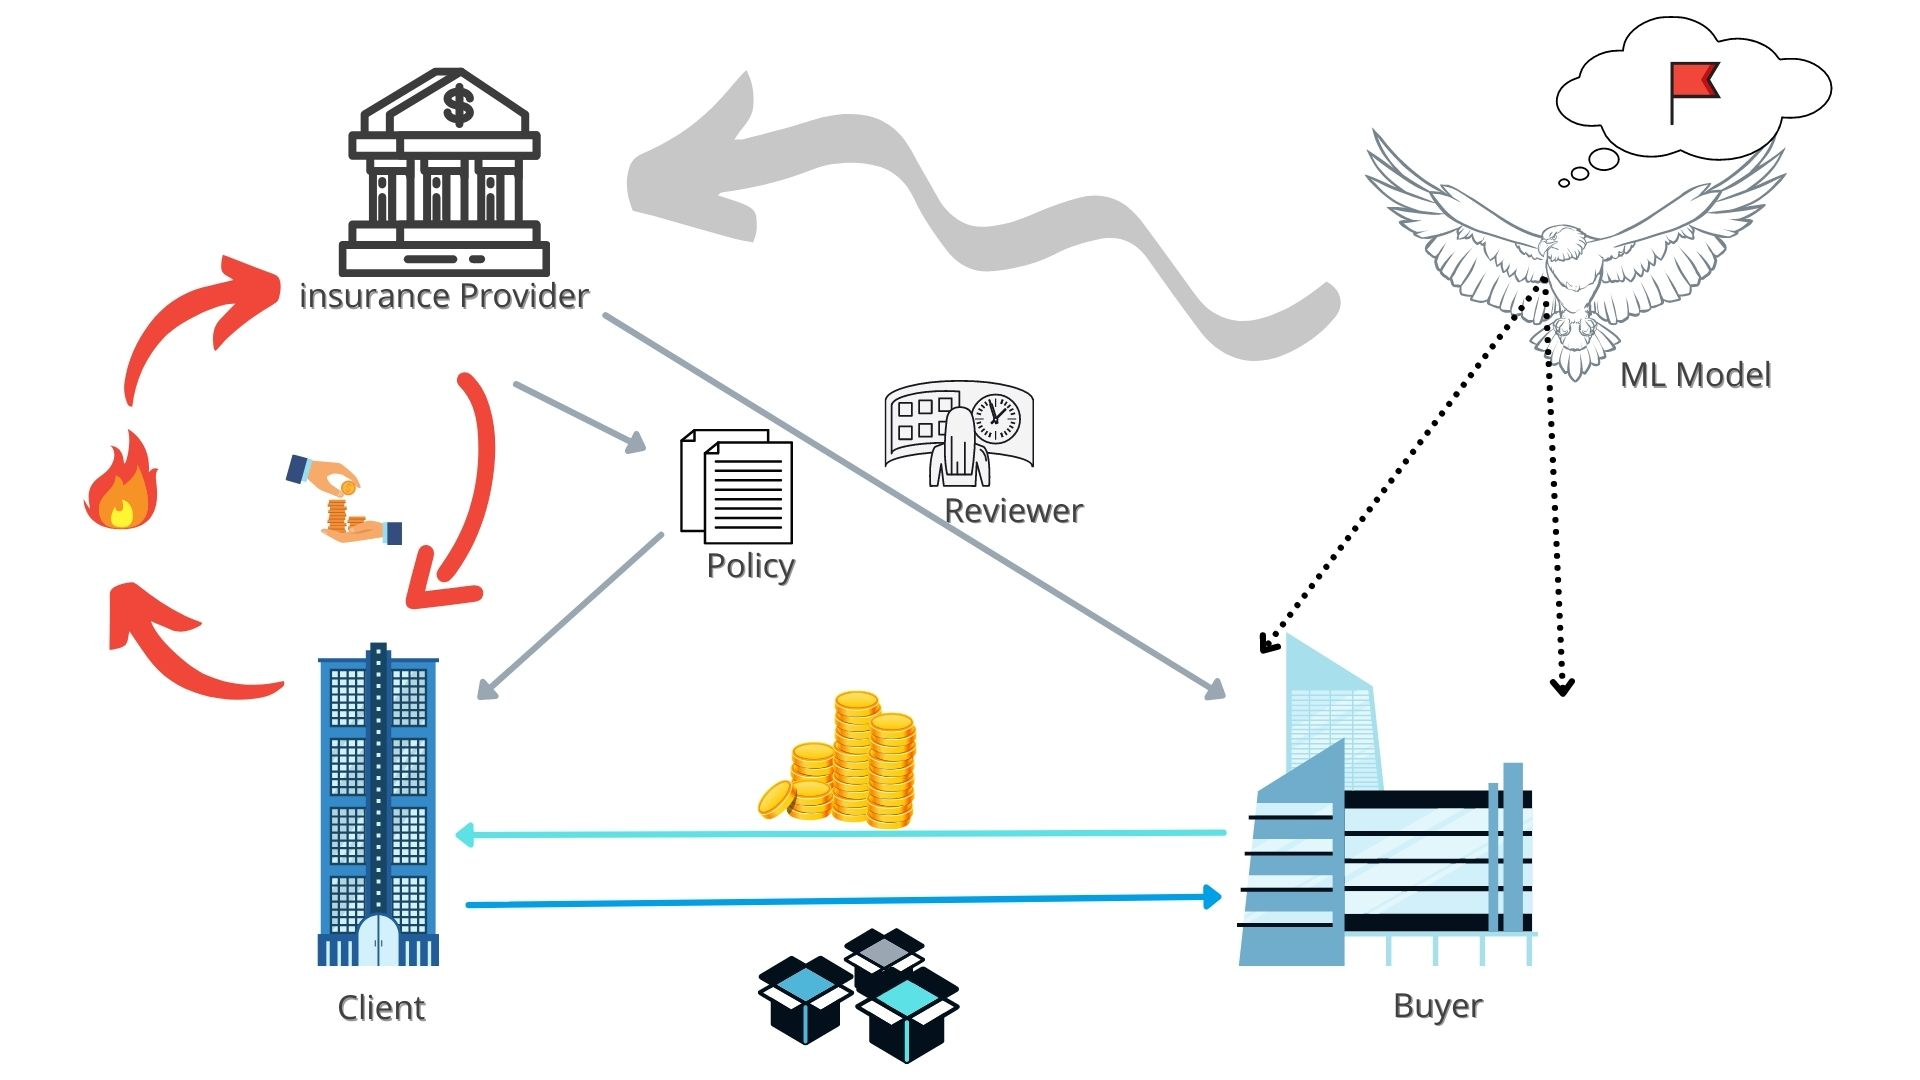
\includegraphics[width=\linewidth]{figures/monitor_buyers.jpg}
    \caption{Trade credit issuing process}
    \label{fig:trade_credit}
\end{figure}

A joint data-driven technique and machine learning algorithms approach are used in this work for this classification task. Before the classification step, number of new features are generated or engineered from the internal company data. the insight from the experts are considered first, then from the historical reports the data driven method was used to prepare a dataset to train the desired model. Based on statistical correlation the important features are selected as final features to train various Ensemble models and artificial neural networks are used to get the best out come. \mytodo{refer the the three step flow}

Firs step of data driven approach is to apply the theory of change. As per the theory of change we can find the road map for how to get company information which are most useful. This method also help to find how to archive long time goals along with indicator for improve and track progress. Then its important to get in touch with internal experts to understand what sort of data they are using for daily tasks.

Generally the classifiers perform quite weak due to missing values and imbalance dataset for real life scenarios. The one of the major reason for the missing data is the collected data does not contain enough information, because of he statistical error or some missing values. To obtain more hidden
information, data-driven method generally is a good choice. In the data driven approach hidden features can be found based on feedback from expert

Data-driven decision making means getting the right data to the right model to the right time to improve the model for problem solving. This approach can help the organisation to identify and apply recent trend in data to apply it for finding solutions. 


